\documentclass{article}\usepackage[]{graphicx}\usepackage[]{xcolor}
% maxwidth is the original width if it is less than linewidth
% otherwise use linewidth (to make sure the graphics do not exceed the margin)
\makeatletter
\def\maxwidth{ %
  \ifdim\Gin@nat@width>\linewidth
    \linewidth
  \else
    \Gin@nat@width
  \fi
}
\makeatother

\definecolor{fgcolor}{rgb}{0.345, 0.345, 0.345}
\newcommand{\hlnum}[1]{\textcolor[rgb]{0.686,0.059,0.569}{#1}}%
\newcommand{\hlstr}[1]{\textcolor[rgb]{0.192,0.494,0.8}{#1}}%
\newcommand{\hlcom}[1]{\textcolor[rgb]{0.678,0.584,0.686}{\textit{#1}}}%
\newcommand{\hlopt}[1]{\textcolor[rgb]{0,0,0}{#1}}%
\newcommand{\hlstd}[1]{\textcolor[rgb]{0.345,0.345,0.345}{#1}}%
\newcommand{\hlkwa}[1]{\textcolor[rgb]{0.161,0.373,0.58}{\textbf{#1}}}%
\newcommand{\hlkwb}[1]{\textcolor[rgb]{0.69,0.353,0.396}{#1}}%
\newcommand{\hlkwc}[1]{\textcolor[rgb]{0.333,0.667,0.333}{#1}}%
\newcommand{\hlkwd}[1]{\textcolor[rgb]{0.737,0.353,0.396}{\textbf{#1}}}%
\let\hlipl\hlkwb

\usepackage{framed}
\makeatletter
\newenvironment{kframe}{%
 \def\at@end@of@kframe{}%
 \ifinner\ifhmode%
  \def\at@end@of@kframe{\end{minipage}}%
  \begin{minipage}{\columnwidth}%
 \fi\fi%
 \def\FrameCommand##1{\hskip\@totalleftmargin \hskip-\fboxsep
 \colorbox{shadecolor}{##1}\hskip-\fboxsep
     % There is no \\@totalrightmargin, so:
     \hskip-\linewidth \hskip-\@totalleftmargin \hskip\columnwidth}%
 \MakeFramed {\advance\hsize-\width
   \@totalleftmargin\z@ \linewidth\hsize
   \@setminipage}}%
 {\par\unskip\endMakeFramed%
 \at@end@of@kframe}
\makeatother

\definecolor{shadecolor}{rgb}{.97, .97, .97}
\definecolor{messagecolor}{rgb}{0, 0, 0}
\definecolor{warningcolor}{rgb}{1, 0, 1}
\definecolor{errorcolor}{rgb}{1, 0, 0}
\newenvironment{knitrout}{}{} % an empty environment to be redefined in TeX

\usepackage{alltt}
\usepackage{hyperref}
\usepackage{amsmath}
%\usepackage[super]{nth}
\IfFileExists{upquote.sty}{\usepackage{upquote}}{}
\begin{document}

\begin{knitrout}
\definecolor{shadecolor}{rgb}{0.969, 0.969, 0.969}\color{fgcolor}\begin{kframe}
\begin{alltt}
\hlcom{### Load libraries}
\hlcom{# Vizualization}
\hlkwd{library}\hlstd{(ggplot2)}
\hlkwd{library}\hlstd{(corrplot)}

\hlcom{# Models}
\hlkwd{library}\hlstd{(Rtsne)} \hlcom{# t-Distributed Stochastic Neighbor Embedding}
\hlkwd{library}\hlstd{(e1071)} \hlcom{# SVM model}

\hlcom{# Evaluation}
\hlkwd{library}\hlstd{(caret)} \hlcom{# Cross-Validation}
\hlkwd{library}\hlstd{(Metrics)} \hlcom{# RMSE metric}
\end{alltt}
\end{kframe}
\end{knitrout}


\section{Data Preparation}

In this section, we will load the data and explore the formats. 
The dataset contains two files:
\begin{itemize}
    \item{\texttt{train.csv} - containing 81 features extracted from 21263 superconductors together with their own critical temperature}
    \item{\texttt{unique\_m.csv} - the chemical formula for each one of the 21263 conductor}
\end{itemize}

This analysis will use the data contained in the \texttt{train.csv}.


\begin{knitrout}
\definecolor{shadecolor}{rgb}{0.969, 0.969, 0.969}\color{fgcolor}\begin{kframe}
\begin{alltt}
\hlstd{original_data} \hlkwb{<-} \hlkwd{read.csv}\hlstd{(}\hlstr{'Data/train.csv'}\hlstd{)}
\hlkwd{dim}\hlstd{(original_data)}
\end{alltt}
\begin{verbatim}
## [1] 21263    82
\end{verbatim}
\end{kframe}
\end{knitrout}

The structure of the data is of the form 81 features, with the $82^{\text{th}}$ column as the target variable, and 21263 instances. The first feature column represents the number of elements the materials have. Then the rest of the 80 columns are based on the following properties with their corresponding units:

\begin{itemize}
\item{\textbf{Atomic Mass} - Atomic Mass Unit (AMU) - Total proton and neutron rest masses}
\item{\textbf{First Ionization Energy} - kilo-Joules per mole ($\frac{kJ}{mol}$) - Energy required to remove the a valence electron}
\item{\textbf{Atomic Radius} - Picometer (pm) - Calculated atomic radius}
\item{\textbf{Density} - Kilograms per meters cubes ($\frac{kg}{m^3}$) - Density at standard temperature and pressure}
\item{\textbf{Electron Affinity} - kilo-Joules per mole ($\frac{kJ}{mol}$) - Energy required to add an electron to a neutral atom}
\item{\textbf{Fusion Heat} - kilo-Joules per mole ($\frac{kJ}{mol}$) - Energy to change from solid to liquid without temperature change}
\item{\textbf{Thermal Conductivity} - Watts per meter Kelvin ($\frac{W}{mK}$) - Thermal conductivity coefficient $\kappa$}
\item{\textbf{Valence} - \# - Typical number of chemical bonds formed by the element}
\end{itemize}

For each one of the enumerated properties, the following measures make up the 80 columns of the data:

\begin{itemize}
\item{\textbf{Mean} = $\mu = \frac{\sum{e_i}}{n}$}
\item{\textbf{Weighted Mean} = $v = \sum{p_i\times e_i}$}
\item{\textbf{Geometric Mean} = $\sqrt[n]{\prod{e_i}}$}
\item{\textbf{Weighted Geometric Mean} = $\prod{e_i^{p_i}}$}
\item{\textbf{Entropy} = $-\sum{w_iln(w_i)}$}
\item{\textbf{Weighted Entropy} = $-\sum{A_iln(A_i)}$}
\item{\textbf{Range} = $e_{\mbox{max}} - e_{\mbox{min}}$}
\item{\textbf{Weighted Range} = $p_{\mbox{max}}e_{\mbox{max}} - p_{\mbox{min}}e_{\mbox{min}}$}
\item{\textbf{Standard Deviation} = $\sqrt{\frac{\sum{(e_i - \mu)^2}}{n}}$}
\item{\textbf{Weighted Standard Deviation} = $\sqrt{\sum{p_i(e_i - v)^2}}$}
\end{itemize}

Where $e_i$ is the property value for the element $i$ of the material, $n$ is the number of elements in the material, $p_i$ is the ratio of elements in the material, $w_i$ is the fraction of the total property value, and $A_i = \frac{p_iw_i}{\sum{p_jw_j}}$


With further analysis, we can see that there are no missing data and that the data type of all of the instances is numerical (3 integers, and 79 continuous). Note that the 3 integer variables will not be transformed into categorical variables. So, no changes will be made and no column will be removed as all of them will be providing information on the target variable.



\section{Exploratory Data Analysis}
In this section, we will try to understand some of the relations between the target variable and the predictors.

\subsection{Target variable}
It is critical to consider the distribution of the target variable, namely the critical temperature. In Figure \ref{histo}, the values for the critical temperature is left-skewed, with the data trending towards 0K, meaning the temperatures are mostly low. Yet with a tail beyond 175K indicating the existence of elements with critical temperature more accessible in practical applications. Now, we will look to see if the entry with highest temeprature is worth keeping for our analysis.

\begin{figure}[h!]
\begin{knitrout}
\definecolor{shadecolor}{rgb}{0.969, 0.969, 0.969}\color{fgcolor}

{\centering 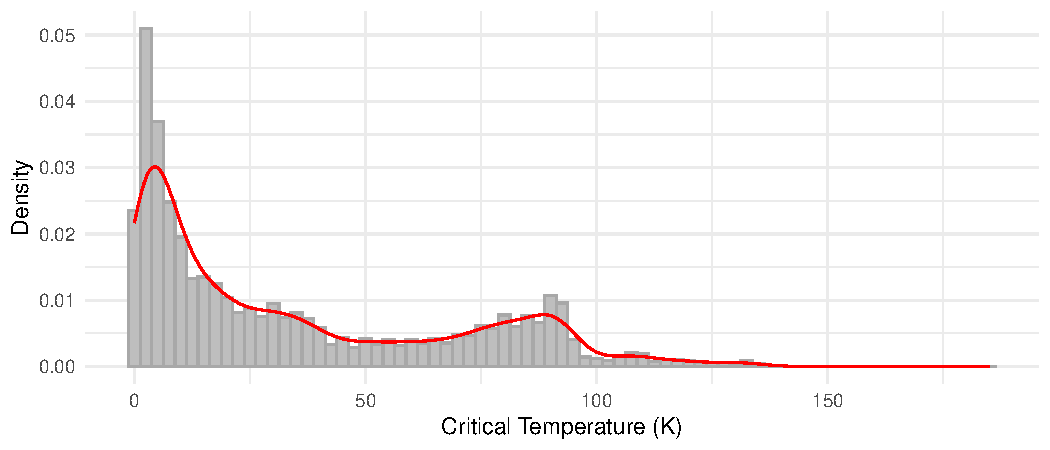
\includegraphics[width=\maxwidth]{figure/unnamed-chunk-3-1} 

}


\end{knitrout}
\caption{Ditribution of Critical Temperature values}
\label{histo}
\end{figure}

The $1.5\cdot IQR$ rule will be used to determine if the entry with the critical temperature 185K is an outlier.

\begin{knitrout}
\definecolor{shadecolor}{rgb}{0.969, 0.969, 0.969}\color{fgcolor}\begin{kframe}
\begin{verbatim}
##      Min.   1st Qu.    Median      Mean   3rd Qu.      Max. 
##   0.00021   5.36500  20.00000  34.42122  63.00000 185.00000
\end{verbatim}
\end{kframe}
\end{knitrout}

$$Q_3 + 1.5 \cdot IQR = Q_3 + 1.5 \cdot (Q_3 - Q_1) = 63 + 1.5 \cdot (63 - 5.365) = 149.4525$$

Conform the $1.5 \cdot IQR$ rule, the entry with the critical temperature 185K is an outlier. Although, looking for the material, it turns out to be hydrogen sulphide, which is one of the superconductors with the highest critical temperature. Additionally, the purpose of the analysis is to give the posibility to discover warmer superconductors. Therefore, the entry will not be removed.


\subsection{Feature Engineering}
Due to the large number of features, it is worth applying dimension reduction algorithms and looking further into the data structure. The algorithms we will use are: 

\begin{enumerate}
    \item t-Distributed Stochastic Neighbour Embedding (t-SNE)
    \item Principal Component Analysis (PCA)
    \item Corrolation Clustering
    \item Hierarchical Clustering
    \item Random Forest
    \item Gradient Boosting
\end{enumerate}


\subsubsection{t-Distributed Stochastic Neighbour Embedding}
The first method to use for dimension reduction is t-distributed stochastic neighbour embedding or t-SNE. This algorithm will take the high-dimensional data points and reduce them to a 2D dimension for better visualisation. This means that it will transform the 81 features of the data into 2 features so the relationship between the entries is preserved.


The main steps to the t-SNE algorithm are:

\begin{enumerate}
    \item Compute High-Dimensional Similarities
    
        The high-dimensional similarity refers to the calculation of the probability of an entry choosing another entry as its neighbour. The probability is calculated between each two points using the Gaussian Distribution as such:
       $$p_{i|j} = \frac{exp(-\frac{||x_i - x_j||^2}{2\sigma_i^2})}{\sum_{k \neq i} exp(- \frac{||x_i - x_k||^2}{2\sigma_i^2})}$$

    \item Compute Low-Dimensional Similarities
    \item Optimize the Embedding
\end{enumerate}


 
- t-SNE - What does it do?
-Small introduction and why I am applying it

\section{Comments}
For further studies, I believe it is worth doing analysis on readings at different pressures. As it is seen for the case of hydrogen sulphide $(H_2S)$ reaching superconductivity properties at the critical temperature of 203K when the pressure is 1.5 million bar. Therefore, following this path will save up resources in finding materials that will present superconductivity properties at temperatures closer to room temperature.
- High acuracy is not a target as we want to understand what makes an element with the desired superconductive critical temperature. -\textgreater Focus on the transparency and 


\end{document}
